\documentclass[journal]{IEEEtran}

\usepackage{cite}
\usepackage{graphicx}
\usepackage{array}

\newcommand{\blurb}[1]{\marginpar{{\tt !!!}}{\tt [... #1 ...]}}

\begin{document}

\title{Capture of Individualized Viewers' Interactions in Interactive TV Environments}
\author{Ricardo~Erikson~V.~de~S.~Rosa, 
	Vicente~Ferreira~de~Lucena~Jr.,\IEEEmembership{Member,IEEE,}
	and~Lucas~Carvalho~Cordeiro
	%
\thanks{Ricardo Erikson V. de S. Rosa is with the Graduate Program in Electrical Engineering, Federal University of Minas Gerais, Av. Antônio Carlos 6627, 31270-901, Belo Horizonte, MG, Brazil(e-mail: ricardoerikson@ufmg.br)}%
\thanks{Vicente Ferreira de Lucena Jr. is with the PPGEE, PPGI, and CETELI - Electronics and Information Technology R\&D Center at UFAM, Manaus, Amazonas, Brazil (e-mail: vicente@ufam.edu.br)}%
\thanks{Lucas Carvalho Cordeiro is with the PPGEE-UFAM, and CETELI - Electronics and Information Technology R\&D Center, Manaus, Amazonas, Brazil (e-mail:lucascordeiro@ufam.edu.br)}}

\maketitle

\begin{abstract}
Advances in TV technology have enabled viewers to actively interact with the TV through interactive applications instead of just passively watching TV. Typically, the interactions occur by using a conventional remote control, which is shared by many viewers and hinders the capture of viewers' individual interactions. It is also difficult to identify the context in which the interactions occur, e.g., to manage precisely who is present in the environment and what is being watched on TV. In this paper, it is presented a novel architecture that facilitates the capture of viewers' individual interactions and contextual data in shared TV environments. This architecture uses personal devices as second screen devices with the aim of identifying viewers and capturing their interactions with interactive TV devices. An implementation of this architecture is reported as an audio-visual content rating system for interactive TV.
\end{abstract}

\begin{IEEEkeywords}
Second screen devices, Interactive Television, Viewers' Interactions
\end{IEEEkeywords}

\IEEEpeerreviewmaketitle

\section{Introduction}

TV watching is essentially a social activity, where groups of people with a common interest share the same space and TV set for entertainment or information. After many advances in technologies for interactive TV (iTV), it is possible to develop high-level applications to enrich the watching experience. Thus, the interaction between viewers and TV became more elaborated than simply change channels and adjust sound volume. Many iTV products, such as Google TV, Apple TV and smart TVs from several manufactures have contributed significantly to this scenario, since they carry a wide variety of services, e.g., news, games and shopping.

The data that is collected from viewers during their interactions with iTV services can provide valuable information for iTV personalization, specially when it is individualized and comes from millions of viewers. Unfortunately, the traditional model of interaction between viewer and TV, which uses a conventional remote control (RC), hinders to obtain this individualized data~\cite{Cesar2008}. The only existing remote control is shared by many viewers and it is difficult to manage who is in possession of the remote control at a given moment. Consequently, it is also difficult to provide high quality personalization, since the tastes that were inferred from the users in charge of the RC can be imposed on the tastes of the others.

In this paper it is presented a novel secondary screen architecture to capture individualized viewers' interactions with iTV services. Personal devices (e.g., smartphones and tablets) are used as secondary screens with the aim of capturing personal interactions from each viewer that is actively interacting with the iTV terminal.In addition, the interactive capabilities of personal devices can provide a powerful interface for users~\cite{Lee2013}.

\section{Overview of the Second Screen Architecture}

The overall architecture of the system is presented in \figurename~\ref{fig_architecture}. This architecture consists of tree parts that interact with each other: (1) second screen devices, which are the personal devices; an (2) iTV terminal; and (3) the content provider infrastructure. The CP infrastructure includes an application hosting infrastructure, which comprises the computing resources (e.g., application server, database services and storage services) that are necessary to host web applications. %The dashed arrows represent the data flowing from the viewer to the CP infrastructure, while dotted arrows denote the flow from CP infrastructure to the viewers. The continuous arrows represent the data flow inside the CP infrastructure.

% Trocar essa figura
\begin{figure}[!t]
	\centering
	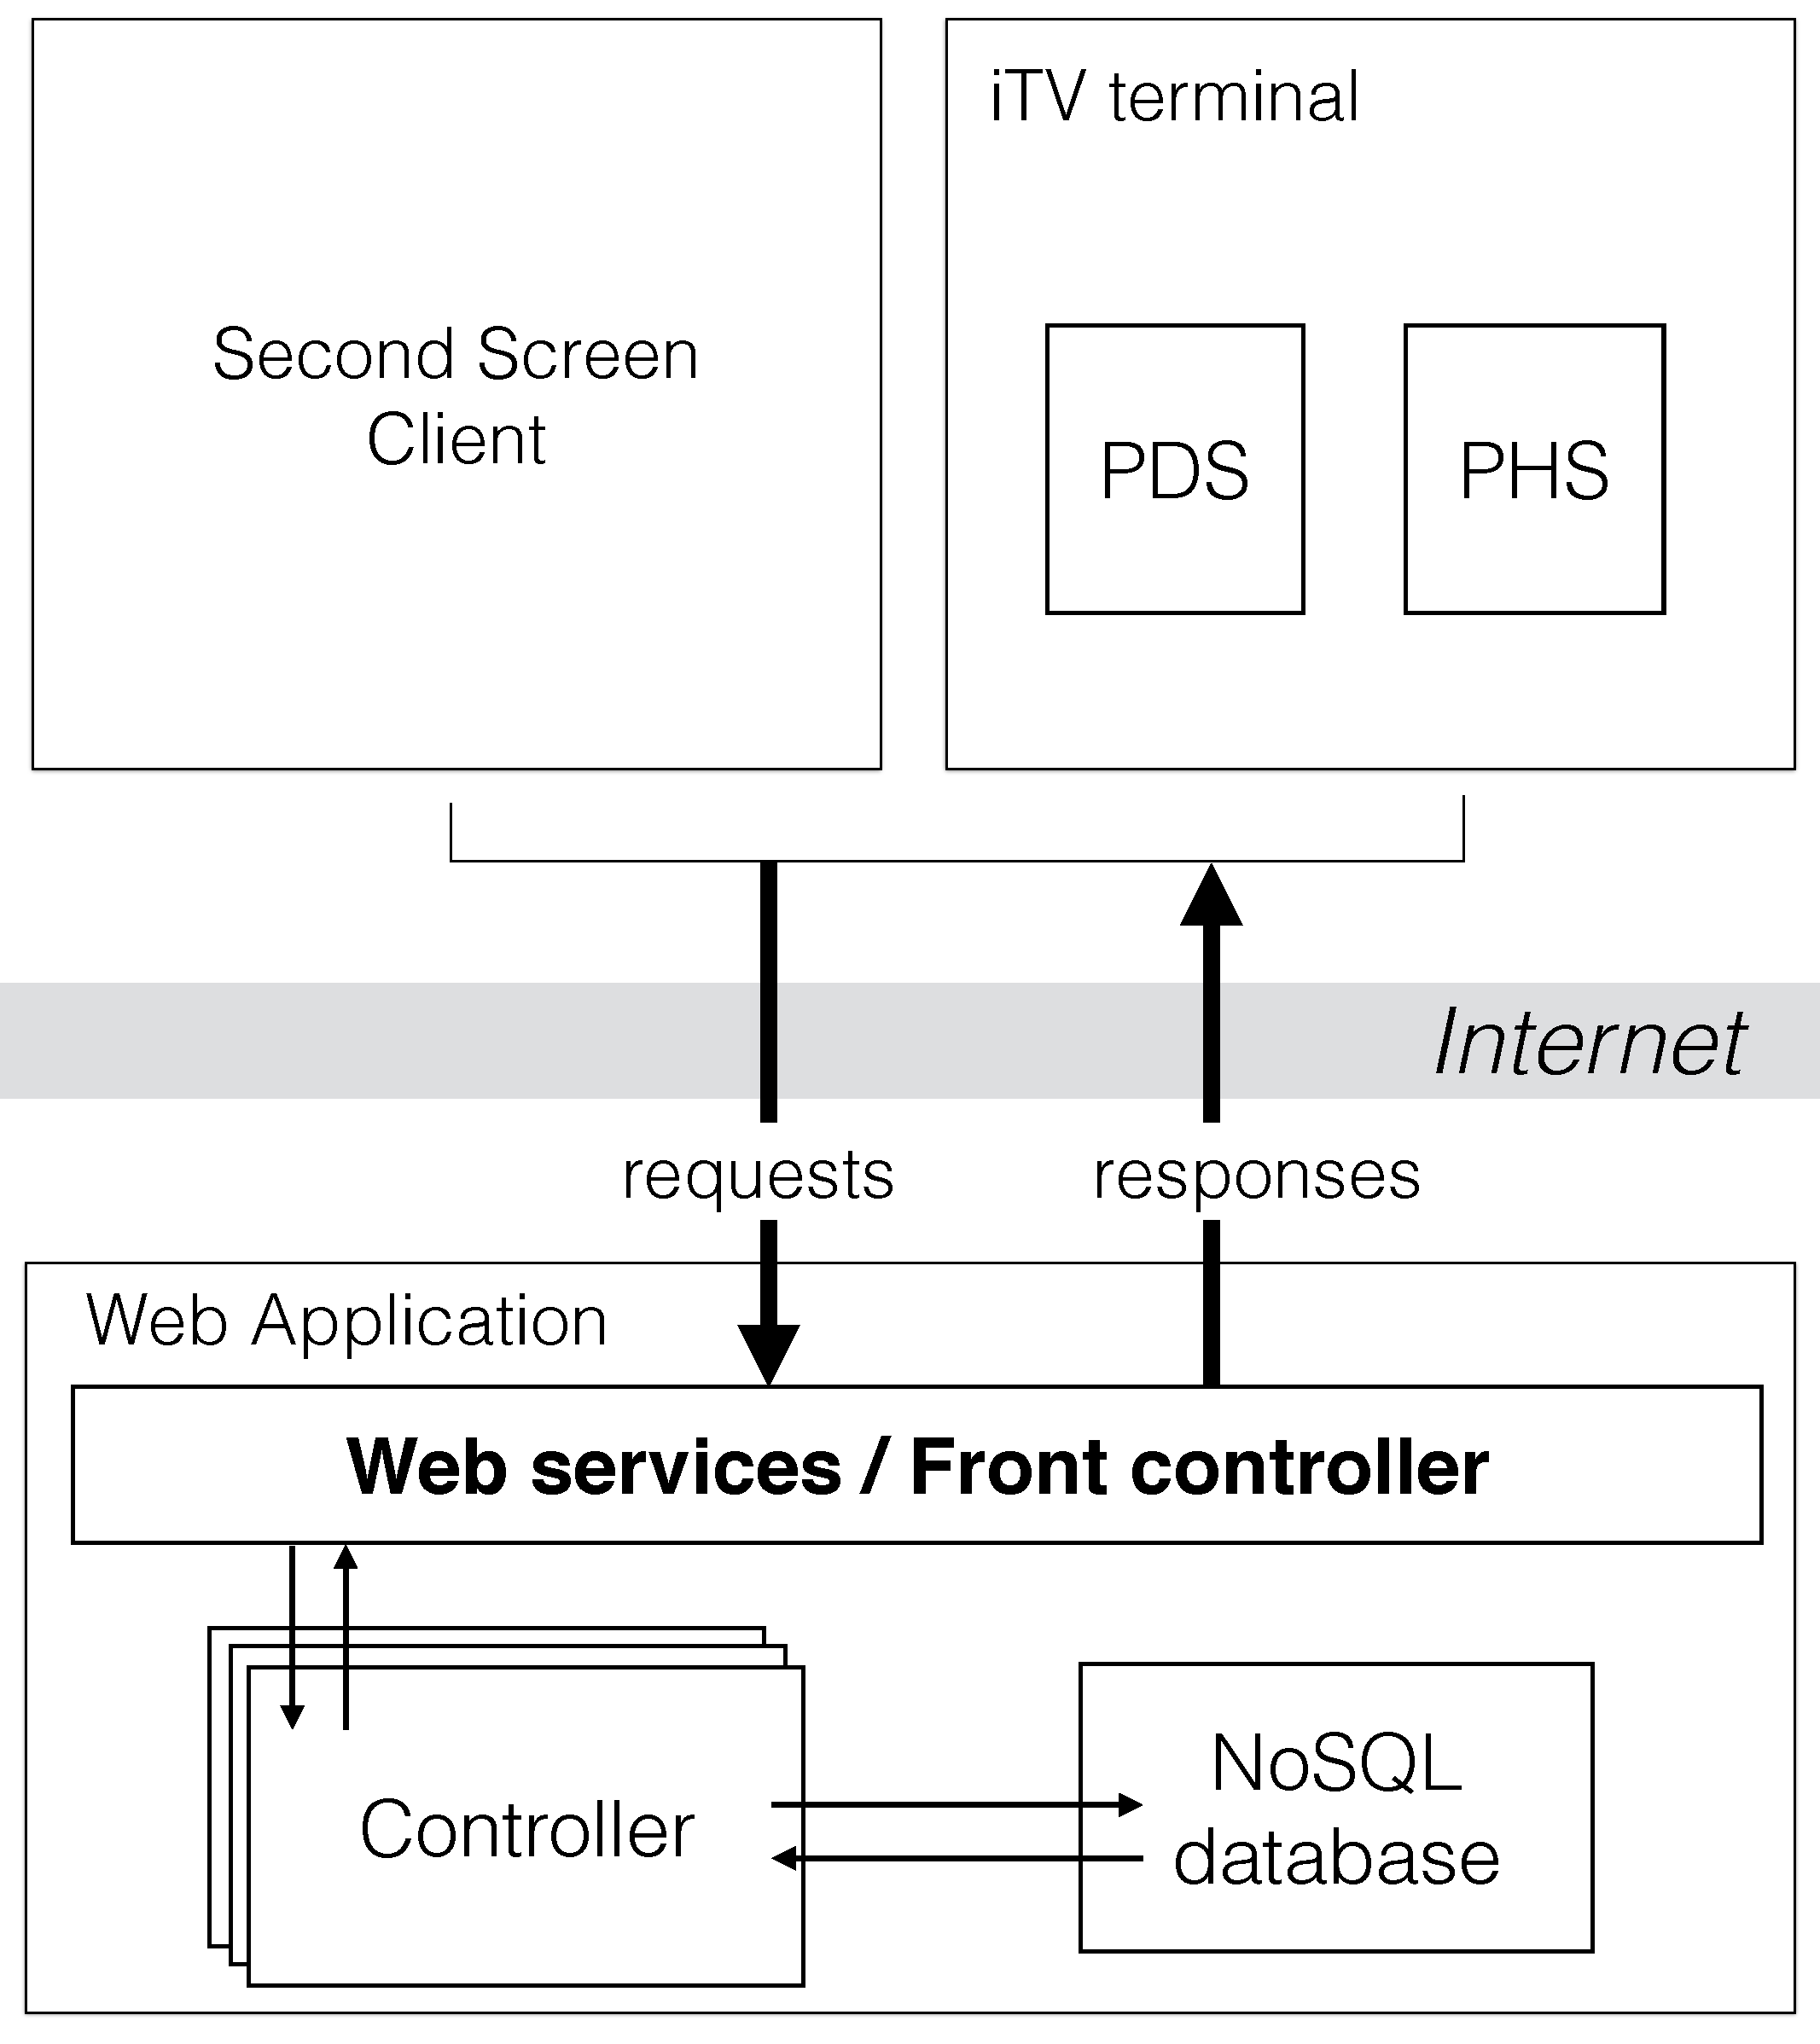
\includegraphics[width=3.5in]{img/architecture-overview.pdf}
	\caption{Architecture to capture audience interactions. The data is captured and stored in the CP infrastructure.}
	\label{fig_architecture}
\end{figure}

A web application is hosted in the application hosting infrastructure. This application contains web services that are designed for interoperability between the second screen devices, the iTV terminal and the CP infrastructure. A authentication mechanism must be provided so that the viewers can connect their second screen devices and interactive TV terminals (e.g., set-top boxes or smart TVs) with an user account. Once the authentication is completed, the second screen device can be used to interact with the iTV terminal. By using the authentication mechanism and considering the second screen client as being a personal device, every user interacting with the iTV terminal can be properly identified.

A presence service detects physically nearby second screen devices that have the services necessary to establish a communication with an iTV terminal. This feature is particularly appropriate for the TV environment, once second screen devices are usually connected with an iTV terminal via WiFi.

The second screen devices and iTV terminals have client applications that consume the web services in order to present the content to the viewers. These client applications also use the web services as an interface to send interaction data to the CP. 

% \section{Second Screen Architecture}

% Viewers can use their secondary screen device to interact with TV by evaluating, commenting, sharing, or even recommending TV content to other viewers. The data related to those actions are naturally provided by the viewers, as part of the interaction, when using interactive applications (developed by the CP) installed in their secondary screen devices. The interactions and the contextual data are represented by the audience data, which is sent to CP infrastructure through Internet. Then, a Data Writer service stores the audience data related to each particular viewer and the iTV device.

% The Data Writer service in the application hosting infrastructure consists basically of web services that provide interoperability among secondary screen devices, iTV devices and the CP infrastructure. The main advantage of this approach is the independence of operating system and programming languages used in the personal devices.
 
% Once the audience data is stored, the CP can use this data to derive valuable information about users' tastes. This information can be used to provide personalized content to viewers based on the current context. Thus, the personalized content can be delivered via Internet to the secondary screen device or even to the TV, depending on the context.

% \subsection{Application Hosting Infrastructure}

% The application hosting infrastructure (AHI) consists of a server environment that provides the necessary computing resources to run a web application and make it available to client applications. This infrastructure can be owned by the CP or it can be hired from a third party service provider. As a matter of fact, the web applications hosted in the AHI are responsible for providing the interactive content that can be accessed by the second screen clients. In addition, the web applications offer features to store and to process interaction data obtained from the viewers.

% The TV domain has the potential of facing very different audience ratings. As a result, the amount of viewers using a particular iTV service can drastically change during the day. So, an important requirement for shared iTV services is to dynamically scale up and down the computing resources according to workload demands. Researchers have proposed novel ideas based on cloud-computing environments to tackle this requirement~\cite{Lee2010,Lai2011}. Since the architecture presented in this paper is intended to support a potentially large amount of viewers, the use of a cloud-computing infrastructure is considered in order to handle the requests from client applications.

% \subsection{Web Application}
% \label{ssub_web_application}

% The web applications include the business logic, models and controllers that are necessary for the proper functioning of the second screen client application. The content that is presented in the client can be requested through HTTP requests to web services designed for this purpose. In addition, the data captured by second screen clients in the iTV environment can also be sent to the CP by using HTTP requests. 

% The HTTP requests handling is carried out by using the front controller architectural design pattern~\cite{Buschmann2007}. It is employed to centralize requests processing in a single component, which facilitates the design and implementation of services for different second screen clients. As a result, client applications can access the same service even when they are developed for different operating systems in different programming languages.

% \subsection{iTV Environment}

% The iTV environment consists of an iTV terminal, which can be an set-top box or some iTV terminal with some sort of communication technology e.g., WiFi or Bluetooth. This environment has some services to facilitate the communication with second screen devices. The first one is the Presence Detector Service (PDS), which is in charge of discovering nearby second screen devices. The PDS is connected with another service known as Profile Handler Service (PHS), which aims to perform profile management at each moment when new second screen devices are found in the iTV environment.

% % describe a device to device communication

% \subsection{Second Screen Devices}

% The second screen devices are clients that communicate with the web application in order to provide interactive capabilities with the content being watched in the TV terminal. The communication between second screen clients and the web application is made through HTTP requests to the web services. Basically, there are two types of communication between clients and the web application: retrieval the content from the web server and transmission of the captured interactions to the web server. Since these types communication occurs between client and a web server, Internet connection is required to accomplish the requests.

% The retrieval of content from the web server happens when the client application performs a specially designed HTTP request aiming to obtain the content from a specified resource. The content obtained from this request is then shown by the client application on the second screen device.

% The interactions captured from the viewers are transmitted to the web server by using the same principle of the retrieval of content. A HTTP request is sent to the web service. However, in this case, the request is designed to submit the data to a specified resource in order to be processed by the web application.

\section{Implementation of the iTV Environment using Second Screen}

The architecture described in this paper combines several concepts and technologies, e.g. second screen, interactive television, mobile applications, device to device communication and web technologies. An implementation of this architecture was developed using the Java programming language in both server and client. However, the proposed approach does not require uniquely the Java programming language and its use does not subtract the generality of the architecture. Indeed, the architecture can be implemented in other languages provided that they are compatible with the development platforms.

A open source web framework~\cite{Walls2011} was used to develop the server side of the architecture, i.e., the web application. This framework facilitates the development of the front controller pattern in web-based applications. Thus, all the requests are tunneled through a single entry point, which is an efficient way to implement a command-based mechanism. This mechanism not only routes and dispatches commands to appropriate handlers, but also exposes a flexible and scalable API structure.

Table~\ref{tab_web_services_design} describes the design of the Unified Resource Identifiers (URIs) to provide a mechanism of interaction between second screen devices and the web application. The CRUD\footnote{Create, Read, Update and Delete} operations can be requested by requested by the second screen client by using a proper resource and selecting a proper HTTP method. Thus, the second screen clients can retrieve the content from the server in order to present personalized content to the client.

\begin{table}[!t]
	\label{tab_web_services_design}
	\renewcommand{\arraystretch}{1.3}
	\caption{Description of the strategies to handle CRUD by combining HTTP methods and URIs.}
	\centering
	\begin{tabular}{|l|c|p{3.5cm}|}
		\hline
		\bfseries Resource & \bfseries HTTP Method & \bfseries Description of the operation
		\tabularnewline\hline
		/resource & GET& Retrieves a list of the specified resource 
		\tabularnewline\hline
		/resource/\emph{\{id\}} & GET & Retrieves a specific resource identified by \emph{\{id\}}
		\tabularnewline\hline
		/resource & POST & Creates a new resource 
		\tabularnewline
		\hline
		/resource/\emph{\{id\}} & PUT & Updates a resource identified by \{id\}
		\tabularnewline
		\hline
		/resource/\emph{\{id\}} & DELETE & Deletes a resource identified by \emph{\{id\}}
		\tabularnewline
		\hline
	\end{tabular}
\end{table}

Second screen clients can also perform requests to send content to the web-application. The client application can be designed to track user interactions and 



\section{Conclusions}

The use of personal devices as secondary screens arises as a new trend in TV environments. This paper presents an architecture to accurately capture audience data by using secondary screen devices and iTV devices. This architecture take advantage of the ubiquity and interactive capabilities of secondary screen devices to identify viewers and provide feedback for CPs through viewers' interactions and contextual information. The captured data relates to a single viewer in a given context. By using proper machine learning algorithms, this data can provide valuable information about viewers. Knowing this information can be very useful for CPs to improve their services aiming to increase the audience and to enrich user experience. As an example, CPs can deliver personalized content for a single person as well as for groups of people by using content recommendation algorithms.

An implementation of the architecture that is described in this paper is under development in a commercial cloud computing platform, which plays the role of the application hosting infrastructure. A web application that consists of a content rating system was developed to store  viewers' evaluations toward audio visual content, and a secondary screen client is under development. Some RESTful web services were developed to provide interoperability among the secondary screen devices and the web application. Thus, the interactions that are captured during the use of the secondary screen application are sent to the CP by means of HTTP requests to RESTful web services. Although the secondary screen application is not fully finished yet, some specific features have been tested to capture viewers' interactions as they occur.

The architecture described in this paper is also technically feasible to implement in Digital TV (DTV) systems and can be particularly interesting for CPs in DTV standards, e.g., the Brazilian (ISDB-TB) and the Japanese(ISDB-T). These standards support the use of mobile devices as part of the system. Since the mobile devices support the implementation of the DTV middleware, a cooperative exhibition of the DTV application can be managed with the iTV device, thus enabling the capture of viewers' interactions and contextual data.

\bibliographystyle{IEEEtran}
\bibliography{biblio}

\end{document}